\documentclass[../main.tex]{subfiles}
\begin{document}
\chapter{1D Solutions of TISE}
\section{Bound States}
We would like to find the eigenstates and eigenvalues of the operator $\hat{H}$ for various potentials $U(x)$ as this allows us to express any state $\psi$ as a linear combination of such eigenstates.

When we expand $\hat{H} \chi = E \chi$, we have:
\[
  -\frac{\hbar^2}{2m} \chi''(x) + U(x) \chi(x) = E \chi(x)
\]
So if $U(x)$ is finite, then any eigenfunction $\chi(x)$ must be twice differentiable.
Otherwise, if $U(x)$ is infinite in some regions, then $\chi$ is continuous but $\chi'$ will not be.
\subsection{Infinite Potential Well}
Suppose the potential $U$ is given by:
\[
  U(x) = \begin{cases}
  0 & \text{ if } |x| \leq a \\
  \infty & \text{ if } |x| > a
  \end{cases}
\]
where $a \in \R^{+}$ is some constant.
This is \textit{the infinite potential square well}.

For $|x| > a$, we must have $\chi(x) = 0$ otherwise we would have $U\chi = \infty$.
For $|x| \leq a$, we want to solve:
\[
  \chi'' + \frac{2mE}{\hbar^2} \chi = 0
\]
with the continuity condition $\chi(a) = \chi(-a) = 0$.

If $E < 0$, then we always obtain the null state after applying the continuity conditions.
Thus to look for eigenstates, we must have $E \geq 0$ and so we define $k^2 = \frac{2mE}{\hbar^2} \geq 0$.
In this case, we have:
\[
  \chi'' + k^2 \chi = 0 \implies \chi(x) = A\sin(kx) + B\cos(kx)
\]
for constants $A$ and $B$.

Applying the continuity conditions, we obtain that both $A\sin(ka) = 0$ and $B\cos(ka) = 0$.
We need both of these to hold and $\chi$ to not be identically 0.
Since $\sin(ka)$ and $\cos(ka)$ cannot both be simultaneously 0, there are two options:
There is therefore two options:
\begin{enumerate}
  \item We have $A = 0$ and $B \neq 0$, thus $k_n = n \cdot \frac{\pi}{2a}$ for odd $n \geq 1$.
    Substituting in, we obtain the eigenfunctions:
    \[
      \chi_n(x) = B \cos(k_n x)
    \]
    for odd $n \in \N$.
  \item We have $B = 0$ and $A \neq 0$, thus $k_n = n \cdot \frac{\pi}{2a}$ for even $n \geq 2$.
    Substituting in, we obtain the eigenfunctions:
    \[
      \chi_n(x) = A \sin(k_n x)
    \]
    for even $n \in \N$.
\end{enumerate}
Having found $k_n = n \cdot \frac{\pi}{2a}$ for $n \geq 1$, we can find the eigenvalues $E_n$ for $\hat{H}$:
\[
  E_n = \frac{\hbar^2}{2m} k^2_n = \frac{\hbar^2\pi^2}{8ma^2}n^2 \text{ for } n \geq 1
\]
which are therefore only allowed energy levels for particles in the system.

We would like our stationary states to be normalised and so we can determine $A$ and $B$ by imposing that:
\[
  \int_{-a}^{a} |\chi_n(x)|^2 \d{x} = 1 \implies A = B = e^{i\alpha}\sqrt{\frac{1}{a}} \text{ for some } \alpha \in \R
\]
For convenience, we pick $\alpha = 0$ so that $A, B \in \R$ and so out eigenfunctions will also be real.
Thus the eigenfunctions of $\hat{H}$ with this potential are:
\[
  \chi_n(x) = \begin{cases}
  \sqrt{\frac{1}{a}} \cos\left(\frac{n \pi x}{2a}\right) & \text{ if } n \in \{1, 3, 5, \ldots\} \text{ and } |x| \leq a \\
  \sqrt{\frac{1}{a}} \sin\left(\frac{n \pi x}{2a}\right) & \text{ if } n \in \{2, 4, 6, \ldots\} \text{ and } |x| \leq a \\
  0 & \text{ if } |x| \geq a
  \end{cases}
\]
Graphically, the first three of these, which correspond to the three lowest energy states are:
\begin{center}
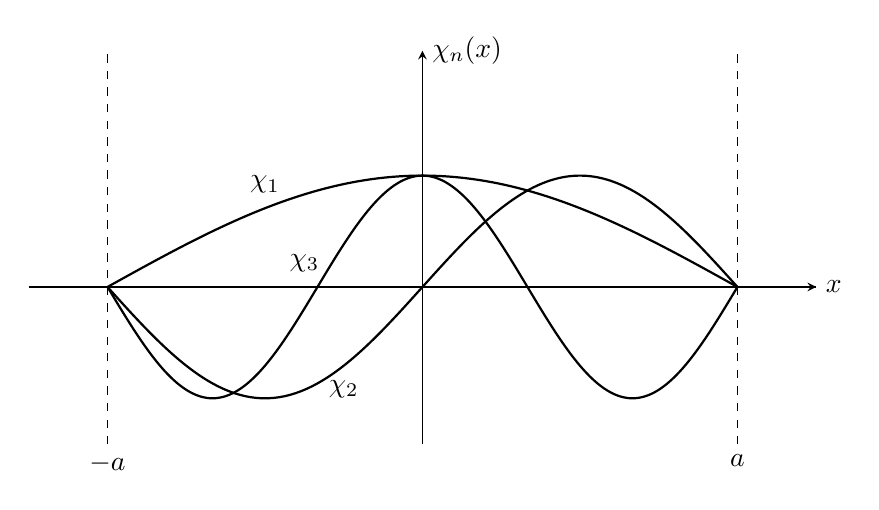
\begin{tikzpicture}[>=stealth]
  \def\aconst{2}
  \draw[->] (0, -2) -- (0, 3) node[right] {$\chi_n(x)$};
  \draw[->] (-5, 0) -- (5, 0) node[right] {$x$};

  \draw[dashed] (-2 * \aconst, -2) node[below] {$-a$} -- (-2 * \aconst, 3);
  \draw[dashed] (2 * \aconst, -2) node[below] {$a$} -- (2 * \aconst, 3);
  \draw[thick] (-5, 0) -- (-2 * \aconst, 0);
  \draw[thick] (2 * \aconst, 0) -- (5, 0);

  \node at (-2, 1.3) {$\chi_1$};
  \node at (-1, -1.3) {$\chi_2$};
  \node at (-1.5, 0.3) {$\chi_3$};
  \begin{scope}[scale=2]
    \draw[thick, domain=-\aconst:\aconst, smooth, variable=\x, samples=100] plot ({\x}, {sqrt(1/\aconst) * cos((pi * \x) / (2 * \aconst) r)});
    \draw[thick, domain=-\aconst:\aconst, smooth, variable=\x, samples=100] plot ({\x}, {sqrt(1/\aconst) * cos((3 * pi * \x) / (2 * \aconst) r)});
    \draw[thick, domain=-\aconst:\aconst, smooth, variable=\x, samples=100] plot ({\x}, {sqrt(1/\aconst) * sin((pi * \x) / (\aconst) r)});
  \end{scope}
\end{tikzpicture}
\end{center}
We see that $\chi_n(x)$ has $n + 1$ zeroes or \textit{nodes}.
As expected for an infinite potential, we see that, $\chi'_n$ is not continuous at $x = \pm a$.
\begin{remark}
  As we increase $n$, the number of turning points of this graph increases until $\chi_n(x)$ looks like a graph that constantly has $|\chi_n|^2 = \frac{1}{a}$, i.e. a uniform probability distribution on $[-a, a]$:
  \begin{center}
  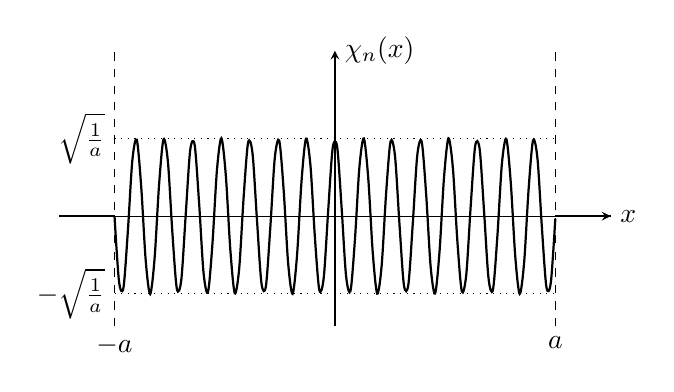
\begin{tikzpicture}[>=stealth, scale=0.7]
    \def\aconst{2}
    \draw[->] (0, -2) -- (0, 3) node[right] {$\chi_n(x)$};
    \draw[->] (-5, 0) -- (5, 0) node[right] {$x$};

    \draw[dashed] (-2 * \aconst, -2) node[below] {$-a$} -- (-2 * \aconst, 3);
    \draw[dashed] (2 * \aconst, -2) node[below] {$a$} -- (2 * \aconst, 3);
    \draw[dotted] (-2 * \aconst, 1.41) node[left] {$\sqrt{\frac{1}{a}}$} -- (2 * \aconst, 1.41);
    \draw[dotted] (-2 * \aconst, -1.41) node[left] {$-\sqrt{\frac{1}{a}}$} -- (2 * \aconst, -1.41);
    \draw[thick] (-5, 0) -- (-2 * \aconst, 0);
    \draw[thick] (2 * \aconst, 0) -- (5, 0);

    \begin{scope}[scale=2]
      \draw[thick, domain=-\aconst:\aconst, smooth, variable=\x, samples=100] plot ({\x}, {sqrt(1/\aconst) * cos((31 * pi * \x) / (2 * \aconst) r)});
    \end{scope}
  \end{tikzpicture}
  \end{center}
  This is consistent with what we would expect for a classical result.
\end{remark}
We note that $\chi_n$ is always an even function for odd $n$ and an odd function for even $n$.
In fact, for any even potential $U$, eigenfunctions of $\hat{H}$ must be either even or odd functions.
\begin{lemma}
  For a quantum system with non-degenerate eigenvalues, if $U(x) = U(-x)$, then the eigenfunctions of $\hat{H}$ have to be either odd or even functions. \label{evenOddEF}
\end{lemma}
\begin{proof}
  Since $U(x) = U(-x)$, the TISE is invariant under $x \mapsto -x$.
  So if $\chi(x)$ is an eigenfunction with eigenvalue $E$, then $\chi(-x)$ is also an eigenfunction with eigenvalue $E$.
  Since the eigenvalues are non-degenerate, $\chi(-x)$ must be $\chi(x)$ up to some constant multiplicative factor $\lambda$, i.e. $\chi(x) = \lambda\chi(-x)$ for some $\lambda \in \C$.

  We then have:
  \[
    \chi(x) = \chi(-(-x)) = \lambda^2 \chi(x) \implies \lambda^2 = 1 \implies \lambda = \pm 1
  \]
  So $\chi(x) = \pm\chi(-x)$, i.e. the eigenfunction is either even or odd.
\end{proof}
\subsection{Finite Potential Well}
We can also have a potential well which is finite.
Suppose the potential $U$ is given by:
\[
  U(x) = \begin{cases}
  0 & \text{ if } |x| \leq a \\
  U_0 & \text{ if } |x| > a
  \end{cases}
\]
where $a \in \R^{+}$ is some constant and $U_0 < \infty$.

We will look for eigenfunctions with $0 \leq E \leq U_0$, the case of $E > U_0$ is an example of a scattering state and will be explored later.
We see that $U(x) = U(-x)$ and so by \cref{evenOddEF}, we need only look for even or odd eigenfunctions.
Here we will look only for even functions, but we will also look for the odd eigenfunctions of this on Example Sheet 2.

Unlike in the case of the infinite potential well, the solution is not necessarily trivial for $|x| \geq 0$ and so we need to solve slightly different cases of the TISE in two regions:
\[
  \begin{cases}
  -\frac{\hbar^2}{2m}\chi''(x) = E \chi(x) & \text{ for } |x| \leq a \\
  -\frac{\hbar^2}{2m}\chi''(x) = (E - U_0)\chi(x) & \text{ for } |x| > a
  \end{cases}
\]
Since $E \geq 0$, we let $k = \sqrt{\frac{2mE}{\hbar^2}}$ so that for $|x| \leq a$ we have:
\[
  \chi''(x) + k^2 \chi(x) = 0 \implies \chi(x) = A \sin(kx) + B \cos(kx)
\]
Since we are looking for even solutions, we must have $A = 0$.

Since $E \leq U_0$, we let $\overline{k} = \sqrt{\frac{2m(U_0 - E)}{\hbar^2}}$ so that for $|x| < a$ we have:
\[
  \chi''(x) - \overline{k}^2 \chi(x) = 0 \implies \chi(x) = Ce^{\overline{k} x} + De^{-\overline{k} x}
\]
We need this function to be square integrable, thus it must be bounded so for $x > a$ we need $C = 0$ and for $x < -a$ we need $D = 0$.
Further, since $\chi(x)$ is even, we must have $C = D$.

In summary:
\[
  \chi(x) = \begin{cases}
  Ce^{\overline{k} x} & \text{ if } x < -a \\
  B\cos(kx) & \text{ if } |x| \leq a \\
  Ce^{-\overline{k} x} & \text{ if } x > a
  \end{cases}
\]
Since $\chi(x)$ must be even, we have $C = D$.

Imposing continuity at $x = \pm a$ gives us:
\[
  Ce^{-\overline{k} a} = B \cos(ka)
\]
and imposing continuity of $\chi'$ at $x = \pm a$ gives us:
\[
  -\overline{k} C e^{-\overline{k} a} = -k B \sin(ka)
\]

To find $C$ and $B$, we first want to find the values of $k$.
Taking the ratio of the continuity equations we obtain:
\[
  k \tan(ka) = \overline{k}
\]
Further, from the definitions of $k$ and $\overline{k}$:
\[
  k^2 + \overline{k}^2 = \frac{2mU_0}{\hbar^2}
\]
Thus we want to find the intersection of the graphs $k \tan(ka) = \overline{k}$ and $k^2 + \overline{k}^2 = \frac{2mU_0}{\hbar^2}$.
Rescaling the variables using $\xi = ka$ and $\eta = \overline{k} a$, we are looking for the intersections of $\xi \tan \xi = \eta$ and $\chi^2 + \eta^2 = r^2_0$ where $r^2_0 = \frac{2mU_0}{\hbar^2}a^2$.
Graphically:
\begin{center}
\begin{tikzpicture}[>=stealth]
  \draw[->] (0, 0) -- (0, 5) node[right] {$\eta$};
  \draw[->] (0, 0) -- (11, 0) node[right] {$\xi$};

  \draw[thick, domain=0:1, smooth, variable=\x, scale=3] plot ({\x}, {\x * tan(\x r)}) node[right] {$\xi \tan \xi$};
  \draw[thick, domain=3.14:3.55, smooth, variable=\x, scale=3] plot ({\x}, {\x * tan(\x r)});
  \clip (0, 0) rectangle (5, 5);
  \draw[thick] (0, 0) circle (3cm);
  \node at (4, 1) {$\xi^2 + \eta^2 = r^2_0$};
\end{tikzpicture}
\end{center}
We will always have at least one intersection, and as the value of $r_0$ increases, we can get any finite number of intersections $p$.

Thus the eigenvalues of $\hat{H}$ correspond to these $p$ intersections:
\[
  E_n = \frac{\hbar^2}{2ma^2} \xi^2_n
\]
where $\xi_n$ are $\xi$-coordinates at the points of intersection for $n \in \{1, \ldots, p\}$.
\begin{remark}[Remarks]
  \begin{enumerate}
    \item We can use the continuity conditions to determine $C$ in terms of $B$ and then impose normalisation to determine $C$.
    \item Because of the exponential terms, these solutions have non-zero probability for $|x| > a$ which is forbidden classically.
  \end{enumerate}
\end{remark}
\subsection{Harmonic Oscillator}
Suppose the potential $U$ is given by:
\[
  U(x) = \frac{1}{2} kx^2 = \frac{1}{2} m\omega^2 x^2
\]
where $k \in \R^{+}$ is the \textit{elastic constant} and $\omega = \sqrt{\frac{k}{m}}$.
Recall from IA Differential equations that in classical mechanics we had:
\[
  \ddot{X}(t) = - \omega^2 X(t) \implies X(t) = A \sin(\omega t) + B \cos(\omega t)
\]
So $\omega$ is the frequency of the analogous classical harmonic oscillator.

However in quantum mechanics, we look for normalised eigenfunctions of $\hat{H}$, i.e. $\chi(x)$ satisfying:
\[
  -\frac{\hbar^2}{2m} \chi''(x) + \frac{1}{2} m \omega^2 x^2 \chi(x) = E \chi(x)
\]
Since $U$ is an even function, by \cref{evenOddEF}, we will only have even or odd eigenfunctions.

Looking for eigenfunctions becomes easier if we perform the change of variables:
\[
  \xi^2 = \frac{m\omega}{\hbar} x^2 \text{ and } \varepsilon = \frac{2E}{\hbar \omega}
\]
which gives:
\[
  -\deriv[2]{}{\xi} \chi(\xi) + \xi^2 \chi(\xi) = \varepsilon \chi(\xi)
\]
\section{Free Particles}
\section{Scattering States}
\end{document}
